%! Author = mariuszindel
%! Date = 25.01.21

\section{Verschlüsselung}

\subsection{Asymetrisch}

\subsubsection{RSA berechnen}
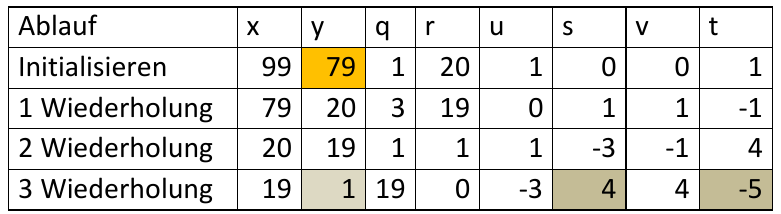
\includegraphics[width=\linewidth]{graphic/extern-reto/RSA.png}
\begin{itemize}
    \item 99 = $\phi(n)$
    \item 79 = privater Schlüssel
    \item 3. Wiederholung \colorbox{gray}{-5}: Inverse, Somit 99 - 5 = 94
    \item 3. Wiederholung \colorbox{lightlightgrey}{1}: ggT
    \item $s = u_{-1} - q_{-1} * s_{-1}$
    \item $t = v_{-1} - q_{-1} * t_{-1}$
    \item Verschlüsselung: $c = m^{Inverse} $ mod $ n$
    \item Entschlüsselung: $m = c^{79}$mod $n$
\end{itemize}
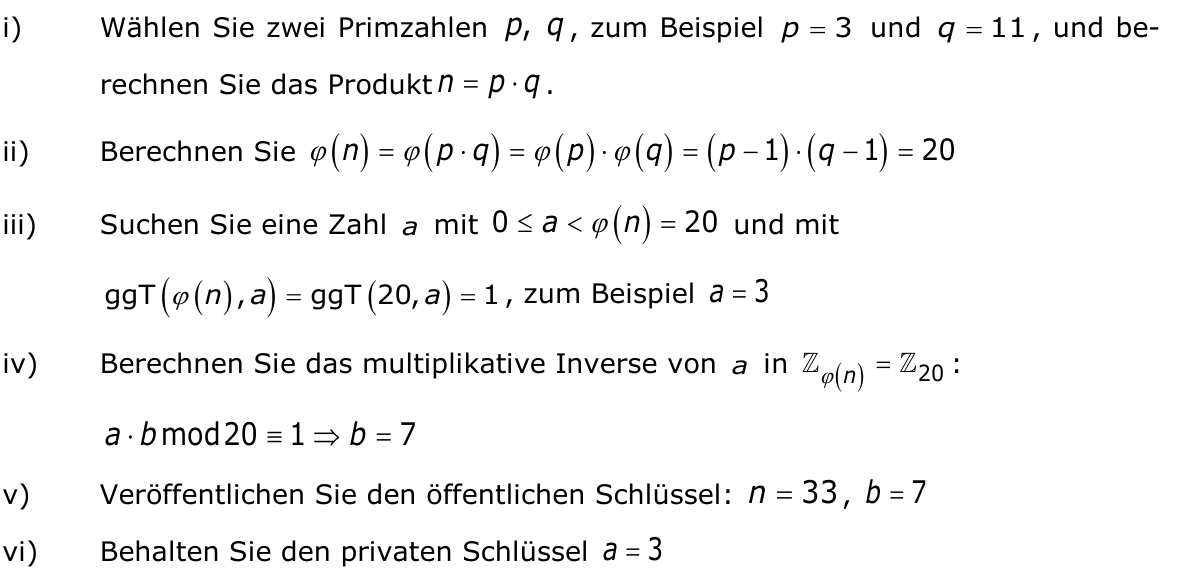
\includegraphics[width=\linewidth]{graphic/extern-reto/RSASchritte.png}

\subsubsection{ n und $\Phi$ berechnen}
Primzahlen p und q müssen gegeben sein
\begin{enumerate}
    \item $n = p \times q$
    \item $\Phi(n)=\Phi(p \cdot q)=(p-1) \cdot(q-1)$
\end{enumerate}

\subsubsection{inversen Schlüssel berechnen}
Zahlen $e_1, e_2 und \Phi(n)$ müssen gegeben sein
\begin{enumerate}
    \item $e_1 \times d_1 mod \Phi(n) = 1$
    \item $e_2 \times d_2 mod \Phi(n) = 1$
\end{enumerate}

\subsubsection{Anz. Schlüssel jeder mit jedem}
$Anz. \times 2 (\rightarrow also = Anz. Paare)$


\subsubsection{Anz. Schlüssel speichern}
Öffentliche Schlüsselbank: 1+1\\
sonst: $Anz. - 1$ öffentliche (der andern) + 1 + 1

\subsection{Symetrisch}
\subsubsection{Anz. Schlüssel jeder mit jedem}
$Anz. / 2 \times (Anz. -1)$


\subsubsection{Anz. Schlüssel speichern}
$Anz. - 1$

\vfill
$$
\columnbreak
